%!TEX root = ../main.tex
%%%%%%%%%%%%%%%%%%%%%%%%%%%%%%%%%%%%%%%%%
%
%LEZIONE 09/03/2016 - TERZA SETTIMANA (2)
%
%%%%%%%%%%%%%%%%%%%%%%%%%%%%%%%%%%%%%%%%%
\chapter{L'integrale di Riemann su più dimensioni}
%%%%%%%%%%%%%%
%INTRODUZIONE%
%%%%%%%%%%%%%%
\section{Introduzione}

\begin{defn}{Rettangolo in \(\R^n\)}{rettangoloRn}\index{Rettangolo in \(\R^n\)}
	Un \emph{rettangolo} in \(\R^n\) si definisce come
	\[
		\mathcal{R}=\Set{(x_1,\ldots,x_n)\in\R^n | a_i\le x_i \le b_i},
	\]
	con \(-\infty<a_i<b_i<+\infty\).
\end{defn}

\begin{oss}
	Le disuguaglianze su \(x_i\) possono essere anche strette.
\end{oss}

\begin{defn}{Misura di un rettangolo}{misuraRettangolo}
	Si definisce \emph{misura di un rettangolo} \(\mathcal{R}\) in \(\R^n\) come
	\[
		\abs{\mathcal{R}}=\prod_{i=1}^n (b_i-a_i).
	\]
\end{defn}

\begin{defn}{Funzione semplice}{funzioneSemplice}\index{Funzione!semplice}
	Una funzione \(s\colon\R^n\to\R\) si definisce \emph{semplice}, o \emph{a gradini}, se è del tipo
	\[
		s(x)=\sum_{j=1}^k a_j 1_{\mathcal{R}_j}(x),
	\]
	dove \(1_{\mathcal{R}_j}\) è la funzione caratteristica del rettangolo \(\mathcal{R}_j\).
\end{defn}

\begin{defn}{Integrale di una funzione semplice}{integraleFunzSemplice}
	Sia \(s\) una funzione semplice, si definisce \emph{intergrale} di \(s\) come
	\[
		\int\limits_{\R^n}s(x)\,\dd x=\sum_{j=1}^k a_j\abs{\mathcal{R}_j}.
	\]
\end{defn}

\begin{pr}
	Se \(s_1,s_2\colon\R^n\to\R\) sono funzioni semplici e \(\a,\b\in\R\), allora
	\begin{itemize}
		\item \(\displaystyle\int\limits_{\R^n}\big( \a\,s_1(x)+\b\,s_2(x) \big)\,\dd x=\a \int\limits_{\R^n}s_1(x)\,\dd x+\b \int\limits_{\R^n}s_2(x)\,\dd x\);
		\item \(\displaystyle\abs*{\int\limits_{\R^n}s_1(x)\,\dd x}\le \int\limits_{\R^n}\abs{s_1(x)}\,\dd x\);
		\item se \(s_1(x)\le s_2(x),\,\fa x\) allora \(\displaystyle\int\limits_{\R^n}s_1(x)\,\dd x\le\int\limits_{\R^n}s_2(x)\,\dd x\).
	\end{itemize}
\end{pr}

\begin{pr}
	Supponiamo che \(s\colon\R^2\to\R\) sia una funzione semplice, allora
	\[
		\int\limits_{\R^2}s(x,y)\,\dd x\,\dd y=\int\limits_\R \dd x\int\limits_\R s(x,y)\,\dd y=\int\limits_\R \dd y\int\limits_\R s(x,y)\,\dd x.
	\]
\end{pr}

\begin{proof}
	Per definizione di funzione semplice
	\[
		s(x,y)=\sum_{j=1}^k a_j 1_{\mathcal{R}_j}(x,y),
	\]
	quindi il suo integrale sarà
	\[
		\int\limits_{\R^2}s(x,y)\,\dd x\,\dd y=\sum_{j=1}^k a_j\abs{\mathcal{R}_j}.
	\]
	Ora
	\[
		\int\limits_\R \dd x \int\limits_\R s(x,y)\,\dd y=\sum_{j=1}^k a_j \int\limits_\R \dd x \int\limits_\R 1_{\mathcal{R}_j}(x,y)\,\dd y,
	\]
	dove \(1_{\mathcal{R}_j}\), congelando la \(x\), è la funzione caratteristica di un intervallo di \(y\), ora
	\[
		\mathcal{R}_j=\Set{(x,y)\in\R^2 | x\in(\a_j,\b_j),y\in(\g_j,\d_j)},
	\]
	quindi \(1_{\mathcal{R}_j}(x,y)=0\) se \(x\notin (\a_j,\b_j)\).
	Quindi
	\[
		\begin{split}
			\sum_{j=1}^k a_j \int\limits_\R \dd x \int\limits_\R 1_{\mathcal{R}_j}(x,y)\,\dd y & =\sum_{j=1}^k a_j \int\limits_\R 1_{(\a_j,\b_j)}(x)(\d_j-\g_j)\,\dd x\\
			& =\sum_{j=1}^k a_j (\d_j-\g_j) \int\limits_\R 1_{(\a_j,\b_j)}(x)\, \dd x\\
			& =\sum_{j=1}^k a_j (\d_j-\g_j)(\b_j-\a_j)\\
			& =\sum_{j=1}^k a_j \abs{\mathcal{R}_j}.\qedhere
		\end{split}
	\]
\end{proof}

\begin{oss}
	In generale questo vale su \(\R^n\) per ogni funzione a scalini.
\end{oss}

\begin{defn}{Funzione Riemann integrabile}{RIntegrabile1}\index{Riemann integrabile}
	Una funzione \(f\colon\R^n\to\R\) si dice \emph{Riemann integrabile} se l'estremo superiore dell'insieme
	\[
		A=\Set{\int\limits_{\R^n}u(x)\,\dd x | u\text{ semplice},u(x)\le f(x),\,\fa x}
	\]
	coincide con l'estremo inferiore dell'insieme
	\[
		B=\Set{\int\limits_{\R^n}v(x)\,\dd x | v\text{ semplice},v(x)\ge f(x),\,\fa x}.
	\]
\end{defn}

\begin{defn}{Funzione Riemann integrabile (equivalente)}{RIntegrabile2}
	Una funzione \(f\colon\R^n\to\R\) si dice \emph{Riemann integrabile} se
	\[
		\fa \e>0\,\ex u,v\colon\R^n\to\R\text{ semplici, con }u(x)\le f(x)\le v(x),\,\fa x\in\R^n,
	\]
	tali che
	\[
		\int\limits_{\R^n}\big[v(x)-u(x)\big]\,\dd x < \e.
	\]
\end{defn}

\begin{teor}{Equivalenza delle definizioni di Riemann integrabilità}{RIntegrabileEquiv}
	Una funzione \(f\colon\R^n\to\R\) è R-integrabile rispetto alla prima definizione se e soltanto se lo è rispetto alla seconda.
\end{teor}

\begin{proof}
	\graffito{\(\Rightarrow)\)}Per la definizione di estremo superiore posso trovare una funzione \(u\) semplice, con \(u\le f\), tale che
	\[
		\int\limits_{\R^n}u(x)\,\dd x\ge\sup A- \frac{\e}{2}.
	\]
	Analogamente trovo una funzione \(v\) semplice, con \(v\ge f\), tale che
	\[
		\int\limits_{\R^n}v(x)\,\dd x\le \inf B+ \frac{\e}{2}.
	\]
	Quindi \(u(x)\le f(x) \le v(x)\) e vale
	\[
		\int\limits_{\R^n}v(x)\,\dd x- \int\limits_{\R^n} u(x)\,\dd x\le \e,
	\]
	in quanto \(\sup A=\inf B\) per ipotesi.

	\graffito{\(\Leftarrow)\)}Dal momento che ogni elemento di \(A\) è minore di ogni elemento di \(B\), per l'assioma di Dedekind, avremo
	\[
		\sup A\le \inf B.
	\]
	Il viceversa segue direttamente dall'ipotesi, infatti
	\[
		\sup A\ge \inf B-\e,
	\]
	dove \(\e\) è piccolo a piacere.
	Quindi, per doppia inclusione, avremo
	\[
		\sup A=\inf B.\qedhere
	\]
\end{proof}

\begin{prop}{Proprietà delle funzioni R-integrabili}{propRIntegrabili}
	Ogni funzione \(f\) Riemann integrabile è limitata e nulla al di fuori di un compatto
\end{prop}

\begin{proof}
	Sia \(f\) una funzione Riemann integrabile.
	Per seconda definizione esistono \(u,v\colon\R^n\to\R\) funzioni semplici tali che
	\[
		u(x)\le f(x)\le v(x).
	\]
	Ma, in quanto semplici, tali funzioni sono per definizione limitate e ovviamente nulle al di fuori di un compatto.
	In particolare la funzione
	\[
		u(x)=\sum_{j=1}^k a_j 1_{\mathcal{R}_j}(x),
	\]
	sarà nulla al di fuori dell'unione degli \(\mathcal{R}_j\).
\end{proof}

\begin{ese}
	Non tutte le funzioni sono R-integrabili, ad esempio
	\[
		D(x)=1_{\Q\cap[0,1]}(x)=
		\begin{cases}
			1 & x\in\Q\cap [0,1]  \\
			0 & \text{altrimenti}
		\end{cases}
	\]
	infatti se \(v(x)\) è una funzione semplice tale che \(v(x)\ge D(x)\), allora
	\[
		\int_0^1 v(x)\,\dd x \ge 1,
	\]
	mentre se \(u(x)\) è semplice tale che \(u(x)\le D(x)\), allora
	\[
		\int_0^1 u(x)\,\dd x\le 0,
	\]
	quindi la definizione di integrabilità non è rispettata.
\end{ese}

\begin{pr}
	Siano \(f,g\colon\R^n\to\R\) due funzioni Riemann integrabili e siano \(\a,\b\in\R\), allora
	\[
		\int\limits_{\R^n}\big[\a\,f(x)+\b\,g(x)\big]\,\dd x=\a \int\limits_{\R^n}f(x)\,\dd x+\b \int\limits_{\R^n}g(x)\,\dd x.
	\]
\end{pr}

\begin{pr}
	Siano \(f,g\colon\R^n\to\R\) due funzioni Riemann integrabili tali che
	\[
		f(x)\le g(x),\,\fa x\in\R^n,
	\]
	allora
	\[
		\int\limits_{\R^n}f(x)\,\dd x\le \int\limits_{\R^n}g(x)\,\dd x.
	\]
\end{pr}

\begin{teor}{Condizione di integrabilità}{condIntegrbilità}
	Sia \(f\colon\R^n\to\R\) una funzione continua e a supporto compatto.
	Allora \(f\) è Riemann integrabile.
\end{teor}

\begin{proof}
	Analoga alla dimostrazione in dimensione uno.
\end{proof}

\begin{prop}{Composizione di una funzione continua con una R-integrabile}{compContInt}
	Sia \(f\colon\R^n\to\R\) una funzione R-integrabile e sia \(\j\colon\R\to\R\) continua, allora
	\[
		\j\circ f,
	\]
	è Riemann integrabile.
\end{prop}

\begin{proof}
	Segue banalmente dal teorema precedente.
\end{proof}

\begin{cor}
	Se \(f\) è R-integrabile, allora
	\begin{itemize}
		\item \(\abs{f}\) è R-integrabile;
		\item \(f^+(x)=\max\big(f(x),0\big)\) è R-integrabile;
		\item \(f^-(x)=\max\big(-f(x),0\big)\) è R-integrabile;
		\item \(e^f,f^2,f^3,\ldots\) sono R-integrabili.
	\end{itemize}
\end{cor}

\begin{proof}
	Basta comporre \(f\) con la corrispondente funzione, ad esempio
	\[
		\abs{f}=\j\circ f,\text{ con }\j\colon\R\to\R,x\mapsto\abs{x}.\qedhere
	\]
\end{proof}

\begin{prop}{Prodotto di funzioni R-integrabili}{prodInt}
	Siano \(f_1,f_2\colon\R^n\to\R\) funzioni R-integrabili, allora
	\[
		g(x)=f_1(x)f_2(x),
	\]
	è R-integrabile.
\end{prop}

\begin{proof}
	Sfruttiamo il quadrato di binomio,
	\[
		f_1(x)f_2(x)=\frac{1}{2}\big[f_1(x)+f_2(x)\big]^2- \frac{1}{2}f_1^2(x)- \frac{1}{2}f_2^2(x),
	\]
	quindi \(g\) è R-integrabile in quanto la somma e il quadrato di funzioni integrabile è integrabile.
\end{proof}

\begin{prop}{Disuguaglianza in modulo}{disModulo}
	Sia \(f\colon\R^n\to\R\) una funzione Riemann integrabile, allora
	\[
		\abs*{\int\limits_{\R^n}f(x)\,\dd x}\le \int\limits_{\R^n}\abs{f(x)}\,\dd x.
	\]
\end{prop}

\begin{defn}{Insieme Peano-Jordan misurabile}{peanoJordan1}\index{Misura di Peano-Jordan}
	Un sottoinsieme \(A\subseteq\R^n\) si dice \emph{Peano-Jordan} misurabile se la funzione caratteristica \(1_A\) di \(A\) è Riemann integrabile.
\end{defn}

\begin{defn}{Insieme Peano-Jordan misurabile (equivalente)}{peanoJordan2}
	Un sottoinsieme \(A\subseteq\R^n\) si dice \emph{Peano-Jordan} misurabile se, comunque preso \(\e>0\), trovo due famiglie finite di rettangoli disgiunti
	\[
		\Set{\mathcal{R}_i^{\text{int}}}_{i=0}^a \qquad\text{e}\qquad\Set{\mathcal{R}_j^\text{est}}_{j=0}^b,
	\]
	tali che
	\begin{itemize}
		\item \(\displaystyle\bigcup_{i=1}^a\mathcal{R}_i^\text{int}\subset A\subset \bigcup_{j=1}^b \mathcal{R}_j^\text{est}\);
		\item \(\displaystyle\sum_{j=1}^b\abs*{\mathcal{R}_j^\text{est}}-\sum_{i=1}^a\abs*{\mathcal{R}_i^\text{int}}\le \e\).
	\end{itemize}
\end{defn}

\begin{teor}{Equivalenza delle definizioni di misura di Peano-Jordan}{equivPeanoJordan}
	Un sottoinsieme \(A\subseteq\R^n\) è Peano-Jordan misurabile rispetto alla prima definizione se e soltanto se lo è rispetto alla seconda.
\end{teor}

\begin{proof}
	\graffito{\(\Leftarrow)\)}Dal momento che i rettangoli \(\mathcal{R}_i^\text{int}\) sono disgiunti, avremo
	\[
		1_{\bigcup_{i=1}^a \mathcal{R}_i^\text{int}}(x)=\sum_{i=1}^a 1_{\mathcal{R}_i^\text{int}}(x),
	\]
	ed analogamente
	\[
		1_{\bigcup_{j=1}^b \mathcal{R}_j^\text{est}}(x)=\sum_{j=1}^b 1_{\mathcal{R}_j^\text{est}}(x).
	\]
	Osserviamo che \(A\subseteq B\implies 1_A\le 1_B\), per cui
	\[
		\sum_{i=1}^a \underbrace{1_{\mathcal{R}_i^\text{int}}(x)}_{u(x)} \le 1_A(x) \le \sum_{j=1}^b \underbrace{1_{\mathcal{R}_j^\text{est}}(x)}_{v(x)}.
	\]
	quindi
	\[
		\int\limits_{\R^n}v(x)\,\dd x- \int\limits_{\R^n}u(x)\,\dd x=\sum_{j=1}^b\abs*{\mathcal{R}_j^\text{est}}-\sum_{i=1}^a\abs*{\mathcal{R}_i^\text{int}}\le \e,
	\]
	ovvero, per la seconda definizione di integrabilità, \(1_A\) è Riemann integrabile.

	\graffito{\(\Rightarrow)\)}Dal momento che \(1_A\) è Riemann integrabile comunque preso \(\e>0\), posso trovare \(\mathcal{R}_i,\mathcal{Q}_j\) e \(\a_i,\b_j\in\R\) tali che
	\begin{itemize}
		\item \(\displaystyle\sum_{i=1}^a \a_i 1_{\mathcal{R}_i} (x)\le 1_A(x) \le \sum_{j=1}^b \b_j 1_{\mathcal{Q}_j}(x)\);\graffito{corrisponde alla seconda definizione di integrabilità}
		\item \(\displaystyle \int\limits_{\R^n}\sum_{j=1}^b \b_j 1_{\mathcal{Q}_j}(x)\,\dd x\le \int\limits_{\R^n}\sum_{i=1}^a \a_i 1_{\mathcal{R}_i}(x)+\e\).
	\end{itemize}
	Mi basterebbe quindi che \(\a_i,\b_j=1\) e che \(\mathcal{R}_i,\mathcal{Q}_j\) siano disgiunti.
	Ma posso facilmente supporre che gli insiemi siano disgiunti in quanto, per ogni eventuale intersezione, posso definire nuovi rettangoli, disgiunti, che ricoprano i rettangoli iniziali.

	Adesso posso supporre \(\a_i,\b_j\in\Set{0,1}\), in quanto, ad esempio, gli \(\mathcal{R}_i\) sono disgiunti, quindi se \(\mathcal{R}_i\subseteq A\) avremo
	\[
		\sum_{i=1}^a \a_i 1_{\mathcal{R}_i}(x)\le 1_A(x) \implies \a_i \le 1,
	\]
	in quanto, preso \(x\in A\), esisterà un unico \(\mathcal{R}_i\) tale che \(x\in\mathcal{R_i}\), ovvero
	\[
		1_{\mathcal{R}_k}(x)=0,\,\fa k\neq i.
	\]
	Posso quindi porre \(\a_i=1\).
	D'altronde se \(\mathcal{R}_i\not\subset A\), avremo \(\a_i\le 0\) e posso quindi prendere \(\a_i=0\).

	Ripetendo il medesimo ragionamento per \(\mathcal{Q}_j\), avremo che
	\[
		\mathcal{Q}_j\subset \setc{A}\implies \b_j\ge 0,
	\]
	quindi pongo \(\b_j=0\).
	\[
		\mathcal{Q}_j \cap A\neq \emptyset \implies \b_j\ge 1,
	\]
	quindi pongo \(\b_j=1\).
	Infine avremo
	\begin{itemize}
		\item \(\displaystyle\sum_{i=1}^a 1_{\mathcal{R}_i}(x)\le 1_A(x)\le \sum_{j=1}^b 1_{\mathcal{Q}_j}(x)\);
		\item \(\displaystyle \int\limits_{\R^n}\sum_{j=1}^b 1_{\mathcal{Q}_j}(x)\,\dd x \le \int\limits_{\R^n}\sum_{i=1}^a 1_{\mathcal{R}_i}(x)\,\dd x+\e\).\qedhere
	\end{itemize}
\end{proof}

\begin{ese}
	Non tutti gli insiemi sono Peano-Jordan misurabili, infatti, da quanto visto in un esempio precedente, l'insieme
	\[
		\Q\cap [0,1],
	\]
	non è P-J misurabile.
\end{ese}

\begin{ese}
	Mostriamo che l'insieme
	\[
		E=\Set{(x,y)\in\R^2:y=0,x\in\Q\cap[0,1]}
	\]
	è P-J misurabile.
	Basta prendere
	\[
		[0,1]\times[-\e/2,\e/2]\supseteq E \qquad\text{con}\qquad\abs{[0,1]\times[-\e/2,\e/2]}=\e,
	\]
	e
	\[
		\Set{1/2}\times\Set{0}\subseteq E \qquad\text{con}\qquad\abs{\Set{1/2}\times\Set{0}}=0.
	\]
	Che soddisfano la seconda definizione di misura.
\end{ese}
%%%%%%%%%%%%%%%%%%%%%%%%%%%%%%%%%%%%%%%%%%
%
%LEZIONE 15/03/2016 - QUARTA SETTIMANA (1)
%
%%%%%%%%%%%%%%%%%%%%%%%%%%%%%%%%%%%%%%%%%%
\begin{prop}{Misura di Peano-Jordan in due dimensioni}{misuraPJ2}
	Sia \([a,b]\) un intervallo compatto e sia \(f\colon [a,b] \to [0,+\infty)\) una funzione Riemann integrabile.
	Allora
	\[
		A=\Set{(x,y)\in\R^2 | x\in [a,b], 0 \le y \le f(x)},
	\]
	è Peano-Jordan misurabile e vale
	\[
		\abs{A} = \int_a^b f(x)\,\dd x.
	\]
\end{prop}

\begin{proof}
	Per la definizione di Riemann integrabilità, dato \(\e>0\), trovo
	\[
		a=t_0 < t_1 < \ldots < t_n=b
	\]
	tali che, definiti,
	\begin{gather*}
		s^+(x) = \sum_{i=1}^n 1_{[t_{i-1},t_i)}(t) \sup_{t\in[t_{i-1},t_i)}f(t),\\
		s^-(x) = \sum_{i=1}^n 1_{[t_{i-1},t_i)}(t) \inf_{t\in[t_{i-1},t_i)}f(t),
	\end{gather*}
	si ha
	\[
		\int_a^b \big[s^+(x)-s^-(x)\big]\,\dd x < \e.
	\]
	Ora mi basta prendere gli stessi rettangoli per soddisfare la definizione di Peano-Jordan misurabilità.
	Pongo quindi
	\begin{gather*}
		\mathcal{R}_i^\text{int} = [t_{i-1},t_i) \times \big[0,\inf_{t\in[t_{i-1},t_i)} f(t)\big],\\
		\mathcal{R}_i^\text{est} = [t_{i-1},t_i) \times \big[0,\sup_{t\in[t_{i-1},t_i)} f(t)\big].
	\end{gather*}
	Quindi, per definizione, avremo
	\[
		\bigcup_{i=1}^n \mathcal{R}_i^\text{int} \subseteq A \subseteq \bigcup_{i=1}^n \mathcal{R}_i^\text{est},
	\]
	e
	\[
		\sum_{i=1}^n \abs*{\mathcal{R}_i^\text{est}} - \sum_{i=1}^n \abs*{\mathcal{R}_i^\text{int}} = \int_a^b \big[s^+(x)-s^-(x)\big]\,\dd x < \e,
	\]
	che corrisponde alla seconda definizione di misura di Peano-Jordan.
\end{proof}

\begin{teor}{Operazioni sugli insiemi P-J misurabili}{operazioniPJ}
	Siano \(A,B \subseteq \R^n\) insiemi Peano-Jordan misurabili, allora
	\begin{itemize}
		\item \(A \cap B\);
		\item \(A \cup B\);
		\item \(A \setminus B\),
	\end{itemize}
	sono Peano-Jordan misurabili.
\end{teor}

\begin{proof}
	Per definizione avremo che \(1_A(x),1_B(x)\) sono Riemann integrabili, da cui:
	\begin{itemize}
		\item \(1_{A \cap B}(x) = 1_A(x) 1_B(x)\) che è R-integrabile in quanto prodotto di funzioni R-integrabili.
		      Quindi \(A \cap B\) è P-J misurabile.
		\item \(1_{A \cup B}(x) = 1_A(x) + 1_B(x) - 1_A(x) 1_B(x)\) che è R-integrabile in quanto somma di funzioni R-integrabili.
		      Quindi \(A \cup B\) è P-J misurabile.
		\item \(1_{A \setminus B}(x) = 1_A(x) - 1_A(x) 1_B(x)\) che è nuovamente R-integrabile.
		      Quindi \(A \setminus B\) è P-J misurabile.\qedhere
	\end{itemize}
\end{proof}

\begin{oss}
	In generale, se \(A\) è P-J misurabile, il complementare di \(A\) non lo è, in quanto può risultare infinito.
	Il problema non si pone se \(A\) è un sottoinsieme di un compatto e il complementare è preso al suo interno.
\end{oss}

\begin{defn}{Riemann integrabile su un insieme P-J misurabile}{riemannPJ}
	Sia \(A\subset \R^n\) un insieme Peano-Jordan misurabile.
	Diremo che una funzione \(f\colon A \to \R\) è Riemann integrabile se la funzione \(\tilde{f}\colon\R^n \to \R\) definita da
	\[
		\tilde{f}(x) = 	\begin{cases}
			f(x) & x\in A    \\
			0    & x\notin A
		\end{cases}
	\]
	è Riemann integrabile.
\end{defn}

\begin{notz}
	Per definizione poniamo
	\[
		\int\limits_A f(x)\,\dd x = \int\limits_{\R^n} \tilde{f}(x)\,\dd x.
	\]
\end{notz}

\begin{oss}
	Presi \(B\subseteq A \subseteq \R^n\) insiemi Peano-Jordan misurabili.
	Se \(f\colon A\to \R\) è una funzione Riemann integrabile, allora \(f\colon B\to \R\) è Riemann integrabile e
	\[
		\int\limits_B f(x)\,\dd x = \int\limits_A f(x) 1_B(x)\,\dd x.
	\]
\end{oss}
%%%%%%%%%%%%%%%%%%%%%%
%FORMULE DI RIDUZIONE%
%%%%%%%%%%%%%%%%%%%%%%
\section{Formule di riduzione}

\begin{defn}{Dominio normale}{dominioNormale}\index{Dominio normale}
	Sia \(E\subset \R^{n+1}\) il dominio di una funzione.
	Diremo che \(E\) è un \emph{dominio normale} se, presi \(A\subseteq \R^n\) un insieme Peano-Jordan misurabile e \(f,g\colon A \to \R\) funzioni Riemann integrabili tali che \(g(x) \le f(x),\,\fa x\in A\), si ha
	\[
		E = \Set{(x,y) \in \R^n \times \R | x\in A, g(x) \le y \le f(x)}.
	\]
\end{defn}

\begin{oss}
	In altre parole un dominio normale è una regione abbastanza regolare da poter essere delimitata da intervalli e grafici di funzione.
\end{oss}

\begin{ese}
	Consideriamo il dominio \(T\), in figura \ref{fig:dominioNormale}, costituito da un cilindroide con "base" \(D\) e compreso tra le funzioni \(a(x,y),b(x,y)\).
	Dalla definizione segue che \(T\) e persino \(D\) sono domini normali, infatti
	\[
		T = \Set{(x,y,z) \in \R^2 \times \R | (x,y) \in D, a(x,y) \le z \le b(x,y)},
	\]
	con
	\[
		D = \Set{(x,y) \in \R \times \R | a \le x \le b, f(y) \le x \le g(y)}.
	\]
	In questo caso si dice che \(T\) è normale al piano \(x\,y\), con \(D\) normale all'asse \(y\).
\end{ese}

\begin{figure}[tp]
	\begin{centering}
		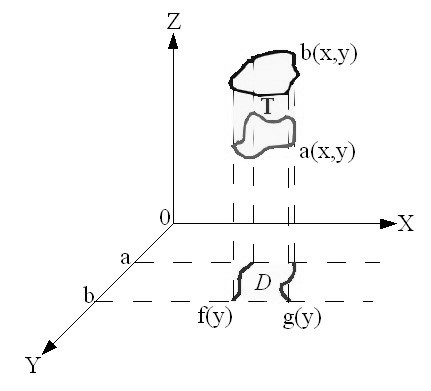
\includegraphics[height = 75mm]{dominioNormale.jpg}
		\caption{Esempio di dominio normale in \(\R^3\) al piano \(x\,y\).}
		\label{fig:dominioNormale}
	\end{centering}
\end{figure}

\begin{prop}{Dominio normale è P-J misurabile}{dominioNormalePJ}
	Siano \(A\subseteq \R^n\) un insieme P-J misurabile e \(f,g\colon A \to \R\) funzioni R-integrabili tali che \(g(x) \le f(x),\,\fa x\in A\).
	Allora il dominio normale
	\[
		E = \Set{(x,y) \in \R^n \times \R | x\in A, g(x) \le y \le f(x)},
	\]
	è Peano-Jordan misurabile e vale
	\[
		\abs{E} = \int\limits_A \big[f(x)-g(x)\big]\,\dd x.
	\]
\end{prop}

\begin{proof}
	Segue generalizzando la proposizione \ref{pr:misuraPJ2}.
\end{proof}

\begin{teor}{Formula di riduzione}{formulaRiduzione}\index{Formula di riduzione}
	Sia \(A\subseteq \R^n\) un insieme Peano-Jordan misurabile e siano \(f,g\colon A \to \R\) funzioni Riemann integrabili tali che \(g(x) \le f(x),\,\fa x\in\ A\).
	Sia
	\[
		E = \Set{(x,y)\in\R^n \times \R | x\in A, g(x) \le y \le f(x)},
	\]
	e sia \(h\colon E \to \R\) una funzione uniformemente continua.
	Allora
	\[
		\int\limits_E h(x,y)\,\dd x\,\dd y = \int\limits_A \dd x\int_{g(x)}^{f(x)}h(x,y)\,\dd y.
	\]
\end{teor}

\begin{proof}
	Non fornita.
\end{proof}

\begin{ese}[dal metodo di Archimede]
	Consideriamo il dominio
	\[
		Z = \Set{(x,y,z) \in \R^3 | x^2+y^2 \le 1, 0\le z \le 2y}.\graffito{Archimede chiamava questa figura "zoccolo".}
	\]
	Dimostriamo che il volume di \(Z\) è pari ad un sesto del volume del cubo circoscritto al cilindro \(x^2+y^2 \le 1\) compreso fra \(0 \le z \le 1\).

	Scriviamo \(Z\) come dominio normale e cerchiamo di applicare il teorema:
	\[
		Z = \Set{(x,y,z) \in \R^3 | (x,y) \in B_1(\bar{0})\cap\{y \ge 0\}, 0 \le z \le 2y}.
	\]
	Quindi avremo, per la formula di riduzione,
	\[
		\iiint\limits_Z \dd x\,\dd y\,\dd z = \iint\limits_{B_1(\bar{0})\cap\{y \ge 0\}}\dd x\,\dd y \int_0^{2y}\dd z = \iint\limits_{B_1(\bar{0})\cap\{y \ge 0\}} 2y\,\dd x\,\dd y.
	\]
	A sua volta \(B_1(\bar{0})\cap\{y \ge 0\}\) risulta essere un dominio normale, nella fattispecie il semicerchio unitario superiore, con
	\[
		B_1(\bar{0})\cap \{y \ge 0\} = \Set{(x,y)\in\R^2 | -1 \le x \le 1, 0 \le y \le \sqrt{1-x^2}},
	\]
	quindi, applicando nuovamente la formula di riduzione, avremo
	\[
		\begin{split}
			\iint\limits_{B_1(\bar{0})\cap\{y \ge 0\}} 2y\,\dd x\,\dd y & = \int_{-1}^1 \dd x \int_0^{\sqrt{1-x^2}} 2y\,\dd y\\
			& =\int_{-1}^1 (1-x^2)\,\dd x \\
			& = \left[x- \frac{x^3}{3}\right]_{-1}^1\\
			& = \frac{4}{3}.
		\end{split}
	\]
	Ora il volume del cubo circoscritto
	\[
		Q = \Set{(x,y,z)\in\R^3 | -1 \le x \le 1, -1 \le y \le 1, -1 \le z \le 1},
	\]
	è \(\abs{Q} = 8\) la cui sesta parte è proprio \(\frac{4}{3}\).
\end{ese}

\begin{ese}
	Preso il dominio \(E = \Set{(x,y,z)\in\R^3 | x^2+y^2+z^2 \le 1}\),
	calcoliamo
	\[
		\int\limits_E \abs{x}\,\dd x\,\dd y\,\dd z.
	\]
	Vogliamo integrare prima rispetto ad \(x\), scriviamo quindi \(E\) come dominio normale:
	\[
		E = \Set{(x,y,z) \in \R^3 | y^2+z^2 \le 1, -\sqrt{1-y^2-z^2} \le x \le \sqrt{1-y^2-z^2}},
	\]
	quindi, applicando la formula di riduzione, avremo
	\[
		\begin{split}
			\iiint\limits_E \abs{x}\,\dd x\,\dd y\,\dd z & = \iint\limits_{\Set{(y,z) | y^2+z^2 \le 1}}\dd y\,\dd z\int_{-\sqrt{1-y^2-z^2}}^{\sqrt{1-y^2-z^2}}\abs{x}\,\dd x\graffito{\(\abs{x}\) è una funzione pari}\\
			& = \iint\limits_{\Set{(y,z) | y^2+z^2 \le 1}}\dd y\,\dd z \, 2\int_0^{\sqrt{1-y^2-z^2}}\abs{x}\,\dd x\\
			& = \iint\limits_{\Set{(y,z) | y^2+z^2 \le 1}}(1-y^2-z^2)\,\dd y\,\dd z\graffito{spezzo l'integrale ricordando che la superficie del cerchio unitario è \(\p\).}\\
			& = \p-2\iint\limits_{\Set{(y,z) | y^2+z^2 \le 1}}z^2\,\dd z\,\dd y.
		\end{split}
	\]
	Scriviamo \(\Set{(y,z) | y^2+z^2 \le 1}\) come dominio normale:
	\[
		\Set{(y,z) | y^2+z^2 \le 1} = \Set{(y,z) | -1 \le y \le 1, -\sqrt{1-y^2} \le z \le \sqrt{1-y^2}},
	\]
	da cui
	\[
		\begin{split}
			\p-2\iint\limits_{\Set{(y,z) | y^2+z^2 \le 1}}z^2\,\dd z\,\dd y & = \p -2\int_{-1}^1 \dd y\int_{-\sqrt{1-y^2}}^{\sqrt{1-y^2}} z^2\,\dd z\\
			& =\p- \frac{4}{3}\int_{-1}^1 (1-y^2)^{\frac{2}{3}}\,\dd y\\
		\end{split}
	\]
	che è un integrale di difficile risoluzione.

	Un procedimento analogo, ma di più facile calcolo, spezzava l'integrale come segue:
	\[
		\int_{-1}^1 \dd x \iint\limits_{E_x}\abs{x}\dd y\,\dd z = 2\int_0^1 x\,\dd x \iint\limits_{E_x}\dd y\,\dd z,
	\]
	con
	\[
		E_x = \Set{(y,z) | x^2+y^2+z^2 \le 1} = \Set{(y,z) | y^2+z^2 \le 1-x^2},
	\]
	che rappresenta nuovamente un cerchio si superficie \(\p(1-x^2)\)\graffito{dalla formula dell'area del cerchio \(\p\,r^2\)}, che ci permette agilmente di calcolare l'integrale come
	\[
		2\int_0^1 x\,\p(1-x^2)\,\dd x.
	\]
\end{ese}

\begin{ese}
	Sul simplesso bidimensionale \(T=\Set{(x,y)\in \R^2 | x,y>0, x+y<1}\), si calcoliamo il valore di
	\[
		\int\limits_T (x^2+\sin y)\,\dd x\,\dd y.
	\]
	Osserviamo, innanzi tutto, che
	\[
		\int\limits_T (x^2+\sin y)\,\dd x\,\dd y = \int\limits_T x^2\,\dd x\,\dd y + \int\limits_T \sin y\,\dd x\,\dd y,
	\]
	scriviamo quindi \(T\) come dominio normale sia rispetto ad \(x\) che rispetto ad \(y\):
	\begin{gather*}
		T = \Set{(x,y) | 0 < x < 1, 0 < y < 1-x},\\
		T = \Set{(x,y) | 0 < y < 1, 0 < x < 1-y}.
	\end{gather*}
	Quindi, applicando la formula di riduzione, avremo
	\[
		\int_0^1 \dd y\int_0^{1-y} x^2\,\dd x + \int_0^1 \dd x \int_0^{1-x} \sin y\,\dd y = \int_0^1 (1-y)^2\,\dd y - \int_0^1 \cos(1-x)\,\dd x,
	\]
	che è un semplice integrale monodimensionale.
\end{ese}

\begin{oss}
	Negli esempi precedenti le ipotesi del teorema erano sempre banalmente soddisfatte, in generale è bene accertarsene.

	In particolare per mostrare l'uniforme continuità può essere utile richiamare proposizioni precedenti quali, ad esempio, la continuità su un compatto.
\end{oss}
%%%%%%%%%%%%%%%%%%%%%%%%%%%%%%%%%%%%%%%%%%
%
%LEZIONE 16/03/2016 - QUARTA SETTIMANA (2)
%
%%%%%%%%%%%%%%%%%%%%%%%%%%%%%%%%%%%%%%%%%%
%%%%%%%%%%%%%%%%%%%%%%%%%%
%CAMBIAMENTO DI VARIABILE%
%%%%%%%%%%%%%%%%%%%%%%%%%%
\section{Cambiamento di variabile}

\begin{teor}{Cambio di variabile}{cambioVariabile}
	Siano \(U,V\subseteq\R^n\) aperti e P-J misurabili.
	Sia \(\j\colon U\to V\) un diffeomorfismo e supponiamo che
	\[
		\sup_{x\in U}\abs{\det \j'(x)}<+\infty.
	\]
	Allora se \(f\colon V\to\R\) è R-integrabile anche \((f\circ \j)\cdot \abs{\det \j'}\) è R-integrabile e si ha
	\[
		\int\limits_V f(y)\,\dd y = \int\limits_U \big(f\circ \j\big)(x) \abs{\det\j'(x)}\,\dd x.
	\]
\end{teor}

\begin{proof}
	Non fornita.
\end{proof}

\begin{oss}
	Come nel caso monodimensionale si può effettuare un cambio di variabile passando direttamente per il differenziale:
	\[
		\int\limits_V f(y)\,\dd y = \int\limits_V f\big(y(x)\big)\,\dd\big(y(x)\big) = \int\limits_U f\big(y(x)\big) \underbrace{\abs*{\det \frac{\pd y}{\pd x}}\,\dd x}_{\dd y}.
	\]
\end{oss}

\begin{prop}{Dilatazione di un dominio}{dilatazioneDominio}
	Sia \(E\subseteq \R^n\) un insieme P-J misurabile.
	Preso \(r>0\) consideriamo l'omotetia
	\[
		r\,E = \Set{y\in\R^n | y = r\,x,x\in E},
	\]
	allora
	\[
		\abs{r\,E} = r^n \abs{E}.
	\]
\end{prop}

\begin{proof}
	Ricordiamo che, per definizione,
	\[
		\abs{r\,E} = \int\limits_{r\,E}\dd y = \int\limits_{\R^n} 1_{r\,E}(y)\,\dd y,
	\]
	dove \(1_{r\,E}\colon\R^n \to \R\) è una funzione ovviamente R-integrabile.
	Consideriamo quindi \(\j\colon \R^n\to\R^n, x\mapsto r\,x\), per cui
	\[
		\j'(x) =\begin{pmatrix}
			r      & 0      & \dots  & 0      \\
			0      & r      & \dots  & 0      \\
			\vdots & \vdots & \ddots & \vdots \\
			0      & 0      & \dots  & r
		\end{pmatrix}
		\implies \abs{\det\j'(x)} = \abs{r^n} = r^n,
	\]
	dove \(r^n\neq 0\) in quanto \(r>0\) per ipotesi.
	Per cui \(\j\) è un diffeomorfismo, possiamo quindi applicare il teorema:
	\[
		\begin{split}
			\abs{r\,E} & = \int\limits_{r\,E}\dd y = \int\limits_{\R^n}1_{r\,E}(y)\,\dd y\\
			& = \int\limits_{\R^n}1_{r\,E}(r\,x)r^n\,\dd x = r^n \int\limits_{\R^n}1_E (x)\,\dd x\graffito{osserviamo che \(r\,x\in r\,E \iff x\in E\)}\\
			& = r^n \abs{E}.\qedhere
		\end{split}
	\]
\end{proof}

\begin{defn}{Trasformazione in coordinate polari}{coordPolari}\index{Coordinate polari}
	Presa \((x,y)\in\R^2\setminus\{(0,0)\}\), esiste una sola coppia \((\r,\q)\in (0,+\infty)\times S^1\) tale che
	\[
		\begin{cases}
			x = \r\cos \q \\
			y = \r\sin \q
		\end{cases}
	\]
	Rimane in tal modo individuato un diffeomorfismo \((x,y)\mapsto(\r,\q)\) la cui funzione inversa è
	\[
		\j\colon(\r,\q)\mapsto (x=\r\cos\q,y=\r\sin\q),
	\]
	detta \emph{trasformazione in coordinate polari}.
\end{defn}

\begin{oss}
	La regolarità della trasformazione è ovvia per la sua definizione. Questo vale anche per la sua inversa, sebbene la sua rappresentazione sia più complicata.
\end{oss}

\begin{notz}
	\(\r\) e \(\q\), che sono funzioni di \((x,y)\), si dicono \emph{coordinate polari} del punto di coordinate cartesiane \((x,y)\).
\end{notz}

\begin{prop}{Calcolo di un integrale mediante coordinate polari}{integraleCoordPolari}
	Sia \(D\subseteq\R^2\) un dominio P-J misurabile e sia \(f\colon D\to\R\) una funzione R-integrabile.
	Se consideriamo \(\j^{-1}(D)\subseteq (0,+\infty)\times S^1\) il dominio la cui immagine tramite trasformazioni in coordinate polari è precisamente \(D\), allora vale
	\[
		\iint\limits_D f(x,y)\,\dd x\,\dd y = \iint\limits_{\j^{-1}(D)} f(\r\cos \q,\r\sin \q)\r\,\dd \r\,\dd \q.
	\]
\end{prop}

\begin{proof}
	Segue direttamente dal teorema, infatti, per definizione
	\[
		\j\colon (0,+\infty)\times S^1 \to \R^2\setminus \{(0,0)\},	\begin{pmatrix}
			\r \\
			\q
		\end{pmatrix}
		\mapsto	\begin{pmatrix}
			x = \r\cos \q \\
			y = \r\sin \q
		\end{pmatrix}
	\]
	per cui
	\[
		\abs*{\det \frac{\pd(x,y)}{\pd(\r,\q)}} = \abs*{\det 	\begin{pmatrix}
				\cos \q & -\r\sin \q \\
				\sin \q & \r\cos \q
			\end{pmatrix}}
		= \abs{\r\cos^2\q + \r\sin^2\q} = \r
	\]
	dove \(\r\neq 0\) in quanto \(\r\in(0,+\infty)\), ovvero ammette inversa \(C^1\) per il teorema della funzione inversa.
	Pertanto \(\j\) soddisfa le ipotesi del cambio di variabile.
	Per ottenere la tesi è quindi sufficiente considerare la restrizione di \(\j\) a \(D\).
\end{proof}

\begin{ese}
	Calcoliamo l'integrale
	\[
		\iint\limits_C \frac{y}{x^2+y^2}\,\dd x\,\dd y,
	\]
	dove \(C=\Set{(x,y)\in\R^2 | y\ge 0, 1 \le x^2+y^2 \le 4}\).

	Per prima cosa è fondamentale rappresentare graficamente il dominio di integrazione, che, come possiamo vedere nella figura \ref{fig:var1}, corrisponde alla superficie compresa fra due semicerchi superiori.

	Essendo un dominio radiale, e presentando nella funzione integranda il termine \(x^2+y^2\), questo integrale si presta molto bene al passaggio in coordinate polari.
	Scriviamo quindi la controimmagine del dominio
	\[
		\j^{-1}(C) = \Set{(\r,\q) | \q\in[0,\p], 1 \le \r \le 2}.
	\]
	Per cui avremo
	\[
		\begin{split}
			\iint\limits_C \frac{y}{x^2+y^2}\,\dd x\,\dd y & = \iint\limits_{\j^{-1}(C)} \frac{\cancel{\r}\sin\q}{\cancel{\r^2}}\cancel{\r}\,\dd\r\,\dd\q\\
			& = \iint\limits_{\j^{-1}(C)}\sin\q\,\dd\r\,\dd\q,
		\end{split}
	\]
	dal momento che \(\j^{-1}(C)\) è già in forma normale, possiamo applicare le formule di riduzione
	\[
		\int_1^2 \dd\r \int_0^\p \sin\q \,\dd\q = \int_1^2 2\,\dd\r = 2.
	\]
\end{ese}

\begin{figure}[tp]
	\begin{centering}
		\includegraphics[height = 75mm]{var1.pdf}
		\caption{Rappresentazione grafica di \(C=\Set{(x,y) | y\ge0, 1\le x^2+y^2\le 4}\).}
		\label{fig:var1}
	\end{centering}
\end{figure}

\begin{ese}
	Calcoliamo l'integrale
	\[
		\iint\limits_B \frac{\dd x\,\dd y}{\sqrt{1-(x^2+y^2)}},
	\]
	dove \(B=\Set{(x,y)\in\R^2 | x^2+y^2\ge \frac{1}{4}, \left(x-\frac{1}{2}\right)^2+y^2 \le \frac{1}{4}}\).

	Dalla rappresentazione grafica di \(B\), figura \ref{fig:var2}, possiamo determinare \(B\) in coordinate polari:
	\[
		\j^{-1}(B) = \Set{(\r,\q) | -\frac{\p}{3} \le \q \le \frac{\p}{3}, \frac{1}{2} \le \r \le \cos\q},
	\]
	dove
	\begin{itemize}
		\item \(\r \ge \frac{1}{2}\) in quanto \(B\) è al di fuori della palla centrata nell'origine di raggio \(\frac{1}{2}\).\\
		\item \(\r \le \cos\q\) in quanto il generico punto sulla palla centrata in \(\frac{1}{2}\) determina, nella semicirconferenza, un triangolo rettangolo inscritto di ipotenusa unitaria e angolo alla base \(\q\).\\
		\item \(-\frac{\p}{3} \le \q \le \frac{\p}{3}\) in quanto l'angolo più esteso determina un triangolo equilatero inscritto nell'intersezione delle due circonferenze.
	\end{itemize}
	Quindi applicando il cambiamento di variabili, otteniamo
	\[
		\iint\limits_B \frac{\dd x\,\dd y}{\sqrt{1-(x^2+y^2)}} = \iint\limits_\j^{-1}(B) \frac{\r}{\sqrt{1-\r^2}}\,\dd\r\,\dd\q,
	\]
	applicando le formule di riduzione,
	\[
		\begin{split}
			\int_{-\frac{\p}{3}}^{\frac{\p}{3}}\dd\q \int_{\frac{1}{2}}^{\cos\q} \frac{\r}{\sqrt{1-\r^2}}\,\dd\r & = \int_{-\frac{\p}{3}}^{\frac{\p}{3}} \left[ -\sqrt{1-\r^2} \right]_{\frac{1}{2}}^{\cos\q}\,\dd\q\\
			& = \int_{-\frac{\p}{3}}^{\frac{\p}{3}} \left( \frac{\sqrt{3}}{2}-\abs{\sin\q} \right)\,\dd\q = 2\int_0^{\frac{\p}{3}} \left( \frac{\sqrt{3}}{2}-\sin\q \right)\,\dd\q\\
			& = 2 \left( \frac{\sqrt{3}}{2}\q+\cos\q \right)_0^{\frac{\p}{3}} = 2 \left( \frac{\sqrt{3}}{2}\frac{\p}{3}+\frac{1}{2}-1 \right)\\
			& = \frac{\sqrt{3}}{3}\p-1
		\end{split}
	\]
\end{ese}

\begin{figure}[tp]
	\begin{centering}
		\includegraphics[height = 75mm]{var2.pdf}
		\caption{Rappresentazione grafica di \(B=\Set{(x,y)\in\R^2 | x^2+y^2\ge \frac{1}{4}, \left(x-\frac{1}{2}\right)^2+y^2 \le \frac{1}{4}}\).}
		\label{fig:var2}
	\end{centering}
\end{figure}

\begin{prop}{Integrale di Gauss}{integraleGauss}\index{Integrale di Gauss}
	La superficie sotto la gaussiana è
	\[
		\int\limits_\R e^{-\frac{x^2}{2}}\,\dd x = \sqrt{2\p}.
	\]
\end{prop}

\begin{proof}
	Consideriamo la palla centrata nell'origine di raggio \(r\),
	\[
		B_r(\bar{0}) = \Set{(x,y)\in\R^2 | x^2+y^2 \le r},
	\]
	e il dominio del quadrato centrato nell'origine di lato \(r\),
	\[
		Q(r) = \Set{(x,y)\in\R^2 | x\in(-r,r),y\in(-r,r)}.
	\]
	Supponiamo che
	\begin{equation}\label{eq:limiteGauss}
		\lim_{r\to+\infty} \int\limits_{B_r(\bar{0})} e^{- \frac{x^2+y^2}{2}}\,\dd x\,\dd y = \lim_{r\to+\infty}\int\limits_{Q(r)} e^{- \frac{x^2+y^2}{2}}\,\dd x\,\dd y.\tag{\(*\)}
	\end{equation}
	In tal caso avremo, applicando le formule di riduzione,
	\[
		\int\limits_{Q(r)}e^{- \frac{x^2+y^2}{2}}\,\dd x\,\dd y = \int_{-r}^r e^{-\frac{x^2}{2}}\,\dd x \int_{-r}^r e^{-\frac{y^2}{2}}\,\dd y \xrightarrow{r} \left( \int\limits_\R e^{-\frac{x^2}{2}}\,\dd x \right)^2,
	\]
	ma abbiamo supposto
	\[
		\int\limits_{Q(r)}e^{-\frac{x^2+y^2}{2}}\,\dd x\,\dd y \cong \int\limits_{B_r(\bar{0})} e^{-\frac{x^2+y^2}{2}}\,\dd x\,\dd y.
	\]
	Passando in coordinate polari otteniamo
	\[
		\j^{-1}\big(B_r(\bar{0})\big) = \Set{(\r,\q) | \r\in(0,r),\q\in S^1},
	\]
	quindi
	\[
		\begin{split}
			\int\limits_{B_r(\bar{0})} e^{-\frac{x^2+y^2}{2}}\,\dd x\,\dd y & =\int\limits_{\j^{-1}\big(B_r(\bar{0})\big)} e^{-\frac{\r^2}{2}}\r\,\dd\r\,\dd\q\\
			& = \int\limits_{S^1}\dd\q \int_0^r \r\,e^{-\frac{\r^2}{2}}\,\dd\r = 2\p \left[ -e^{-\frac{\r^2}{2}} \right]_0^r\\
			& = 2\p \left[ 1-e^{-\frac{\r^2}{2}} \right] \xrightarrow{r} 2\p.
		\end{split}
	\]
	Ovvero, per l'unicità del limite,
	\[
		\left( \int\limits_\R e^{-\frac{x^2}{2}}\,\dd x \right)^2 = 2\p.
	\]
	Resta da dimostrare \eqref{eq:limiteGauss}, per farlo mostriamo che la differenza delle due superfici tende a \(0\):
	\[
		\begin{split}
			\int\limits_{Q(r)\setminus B_r(\bar{0})} e^{- \frac{x^2+y^2}{2}}\,\dd x\,\dd y & \le \int\limits_{B_{\sqrt{2}r}(\bar{0})\setminus B_r(\bar{0})}e^{-\frac{x^2+y^2}{2}}\,\dd x\,\dd y\graffito{passando alle coordinate polari}\\
			& = \int\limits_{\Set{\q\in S^1,r \le \r \le \sqrt{2}r}}e^{-\frac{\r^2}{2}}\r\,\dd\r\,\dd\q\\
			& = \int\limits_{S^1} \dd\q \int_r^{\sqrt{2}r}\r\,e^{-\frac{\r^2}{2}}\,\dd\r\\
			& = 2\p \left[ -e^{-\frac{\r^2}{2}} \right]_r^{\sqrt{2}r}\xrightarrow{r} 0.\qedhere
		\end{split}
	\]
\end{proof}

\begin{oss}
	Tramite le formule di riduzione possiamo calcolare l'integrale di Gauss in \(n\) dimensioni, infatti
	\[
		\begin{split}
			\int\limits_{\R^n} e^{-\frac{\norma{x}^2}{2}}\,\dd x & = \int\limits_{\R^n}e^{-\frac{x_1^2}{2}-\ldots- \frac{x_n^2}{2}}\,\dd x_1\,\ldots\,\dd x_n\\
			& = \int\limits_\R e^{-\frac{x_1^2}{2}}\,\dd x_1 \ldots \int\limits_\R e^{-\frac{x_n^2}{2}}\,\dd x_n = \big(\sqrt{2\p}\big)^n.
		\end{split}
	\]
\end{oss}

\begin{prop}{Volume della sfera \(n\)-dimensionale}{volumeSferaN}
	Consideriamo la generica sfera \(n\)-dimensionale unitaria
	\[
		B_n(1) = \Set{(x_1,\ldots,x_n)\in\R^n | x_1^2+\ldots+x_n^2 \le 1}.
	\]
	Allora, posto \(\w_n\) il valore del suo volume, avremo
	\[
		\w_n = \w_{n-2} \frac{2\p}{n}.
	\]
\end{prop}

\begin{proof}
	Sfruttiamo le formule di riduzione.
	Posto \(x'=(x_3,\ldots,x_n)\) definiamo
	\[
		B^{(x_1,x_2)}(1) = \Set{x'\in\R^{n-2} | (x_1,x_2,x') \in B_n(1)}.
	\]
	Quindi, per costruzione,
	\[
		B^{(x_1,x_2)}(1) = \Set{x'\in\R^{n-2} | \norma{x'}^2 \le 1-(x_1^2+x_2^2)}=B_{n-2}\left(\sqrt{1-(x_1^2+x_2^2)}\right),
	\]
	Posto \(\w_n = \abs{B_n(1)}\), avremo
	\[
		\begin{split}
			\w_n & = \int\limits_{B_n(1)}\dd x_1\,\dd x_2\,\ldots\,\dd x_n = \int\limits_{B_2(1)}\dd x_1\,\dd x_2 \int\limits_{B^{(x_1,x_2)}(1)}\dd x'\\
			& = \int\limits_{B_2(1)}\abs*{B^{(x_1,x_2)}(1)}\,\dd x_1\,\dd x_2.
		\end{split}
	\]
	Ma abbiamo già osservato che \(B^{(x_1,x_2)}(1)=B_{n-2}\left(\sqrt{1-(x_1^2+x_2^2)}\right)\), che corrisponde ad una dilatazione di \(B_{n-2}(1)\) di un fattore \(\sqrt{1-(x_1^2+x_2^2)}\).
	Quindi, dalla proposizione \ref{pr:dilatazioneDominio}, avremo
	\[
		\int\limits_{B_2(1)}\abs*{B^{(x_1,x_2)}(1)}\,\dd x_1\,\dd x_2 = \int\limits_{B_2(1)}\w_{n-2}\big[1-(x_1^2+x_2^2)\big]^{\frac{n-2}{2}}\,\dd x_1\,\dd x_2.
	\]
	Passando in coordinate polari,
	\[
		\begin{split}
			\w_{n-2}\int\limits_{\Set{(\r,\q) | 0<\r<1,\q\in S^1}} (1-\r^2)^{\frac{n-2}{2}}\r\,\dd \r\,\dd \q & = \w_{n-2}\int_0^{2\p}\dd\q\int_0^1 (1-\r^2)^{\frac{n-2}{2}}\r\,\dd\r\\
			& = \w_{n-2}(2\p)\left[ -(1-\r^2)^{\frac{n-2}{2}+1}\frac{1}{n} \right]_0^1\\
			& = \w_{n-2} \frac{2\p}{n}.\qedhere
		\end{split}
	\]
\end{proof}
%%%%%%%%%%%%%%%%%%%%%%%%%%%%%%%%%%%%%%%%%%
%
%LEZIONE 22/03/2016 - QUINTA SETTIMANA (1)
%
%%%%%%%%%%%%%%%%%%%%%%%%%%%%%%%%%%%%%%%%%%
\begin{ese}
	Calcoliamo l'integrale
	\[
		\iint\limits_E \frac{x^2+x\,y^2}{y^3}\,\dd x\,\dd y,
	\]
	dove \(E=\Set{(x,y)\in\R^2 | x \le y \le 2x, x^2 \le y \le 2x^2}\).

	Tramite un disegno si comprende immediatamente che il calcolo di questo integrale in coordinate cartesiane risulta molto difficoltoso.
	Utilizziamo quindi il seguente cambio di variabile definito a partire dalla seguente trasformazione:
	\[
		\j^{-1}	\begin{pmatrix}
			x \\
			y
		\end{pmatrix}
		=	\begin{pmatrix}
			u = \frac{x}{y} \\
			v = \frac{x^2}{y}
		\end{pmatrix}
	\]
	Calcoliamo il dominio nelle nuove coordinate
	\[
		\j^{-1}(I)=\Set{(u,v) | \frac{1}{2} \le u \le 1, \frac{1}{2} \le v \le 1}.
	\]
	Per applicare il teorema del cambio di variabile dobbiamo calcolare lo jacobiano di \(\j\), per farlo calcoliamo quello di \(\j^{-1}\) e applichiamo il teorema della funzione inversa:
	\[
		\abs*{\det \frac{\pd(u,v)}{\pd(x,y)}} = \abs*{\det 	\begin{pmatrix}
				\frac{1}{y}  & -\frac{x}{y^2}   \\
				\frac{2x}{y} & -\frac{x^2}{y^2}
			\end{pmatrix}}
		= \abs*{-\frac{x^2}{y^3} + \frac{2x^2}{y^3}} = \frac{x^2}{y^3}.
	\]
	Da cui
	\[
		\abs*{\det \frac{\pd(x,y)}{\pd(u,v)}} = \left( \frac{\pd(u,v)}{\pd(x,y)} \right)^{-1} = \left. \frac{y^3}{x^2} \right|_{\substack{x = x(u,v)\\y = y(u,v)}} = \frac{v}{u^4}.
	\]
	Applicando il cambio di variabile nell'integrale otteniamo:
	\[
		\begin{split}
			\iint\limits_I \frac{x^2+x\,y^2}{y^3}\,\dd x\,\dd y & = \iint\limits_I \frac{x^2}{y^3}\,\dd x\,\dd y + \iint\limits_I \frac{x}{y}\,\dd x\,\dd y\graffito{\(\frac{x^2}{y^3}\) è l'inverso dello jacobiano di \(\j\)}\\
			& = \iint\limits_{\j^{-1}(I)} \dd u\,\dd v + \iint\limits_{\j^{-1}(I)} u \frac{v}{u^4}\,\dd u\,\dd v,
		\end{split}
	\]
	che è un integrale elementare.
\end{ese}

\begin{defn}{Trasformazione in coordinate cilindriche}{coordCilindriche}\index{Coordinate cilindriche}
	Preso \((x,y,z)\in\R^3\setminus\{(0,0,0)\}\), esiste una sola tripla \((\r,\q,\l)\in (0,+\infty)\times S^1\times \R\) tale che
	\[
		\begin{cases}
			x = \r\cos \q \\
			y = \r\sin \q \\
			z = \l
		\end{cases}
	\]
	Rimane in tal modo individuato un diffeomorfismo \((x,y,z)\mapsto(\r,\q,\l)\) la cui funzione inversa è
	\[
		\j\colon(\r,\q,\l)\mapsto (x=\r\cos\q,y=\r\sin\q,z=\l),
	\]
	detta \emph{trasformazione in coordinate cilindriche}.
\end{defn}

\begin{oss}
	La figura \ref{fig:cordCil} mostra una rappresentazione di un punto in coordinate cilindriche.
\end{oss}

\begin{figure}[tp]
	\begin{centering}
		\includegraphics[height = 75mm]{cordCil.pdf}
		\caption{Rappresentazione del passaggio da coordinate cartesiane a coordinate cilindriche.}
		\label{fig:cordCil}
	\end{centering}
\end{figure}

\begin{notz}
	\(\r,\q\) e \(\l\), che sono funzioni di \((x,y,z)\), si dicono \emph{coordinate cilindriche} del punto di coordinate cartesiane \((x,y,z)\).
\end{notz}

\begin{prop}{Calcolo di un integrale mediante coordinate cilindriche}{integraleCoordCilindriche}
	Sia \(D\subseteq\R^3\) un dominio P-J misurabile e sia \(f\colon D\to\R\) una funzione R-integrabile.
	Se consideriamo \(\j^{-1}(D)\subseteq (0,+\infty)\times S^1\times \R\) il dominio la cui immagine tramite trasformazioni in coordinate cilindriche è precisamente \(D\), allora vale
	\[
		\iiint\limits_D f(x,y,z)\,\dd x\,\dd y\,\dd z = \iiint\limits_{\j^{-1}(D)} f(\r\cos \q,\r\sin \q,\l)\r\,\dd \r\,\dd \q\,\dd \l.
	\]
\end{prop}

\begin{proof}
	La dimostrazione è analoga a quella per le coordinate cilindriche, infatti
	\[
		\j\colon (0,+\infty)\times S^1\times \R \to \R^3\setminus \{(0,0,0)\},	\begin{pmatrix}
			\r \\
			\q \\
			\l
		\end{pmatrix}
		\mapsto	\begin{pmatrix}
			x = \r\cos \q \\
			y = \r\sin \q \\
			z = \l
		\end{pmatrix}
	\]
	per cui
	\[
		\det \frac{\pd(x,y,z)}{\pd(\r,\q,\l)} = \abs*{\det 	\begin{pmatrix}
				\cos \q & -\r\sin \q & 0 \\
				\sin \q & \r\cos \q  & 0 \\
				0       & 0          & 1
			\end{pmatrix}}
		= \abs{\r\cos^2\q + \r\sin^2\q} = \r
	\]
	dove \(\r\neq 0\) in quanto \(\r\in(0,+\infty)\), ovvero ammette inversa \(C^1\) per il teorema della funzione inversa.
	Pertanto \(\j\) soddisfa le ipotesi del cambio di variabile.
	Per ottenere la tesi è quindi sufficiente considerare la restrizione di \(\j\) a \(D\).
\end{proof}

\begin{ese}
	Calcoliamo il volume di
	\[
		E = \Set{(x,y,z) \in \R^3 | x^2+y^2 \le z \le \sqrt{3-2(x^2+y^2)}}.
	\]
	Dalla condizione implicita \(x^2+y^2 \le \sqrt{3-2(x^2+y^2)}\) otteniamo
	\[
		\begin{split}
			(x^2+y^2)^2 \le 3-2(x^2+y^2) & \iff (x^2+y^2)^2+2(x^2+y^2)-3 \le 0\graffito{\(t=x^2+y^2\)}\\
			& \iff t^2+2t-3 \le 0\\
			& \iff -3 \le t \le 1,
		\end{split}
	\]
	ovvero \(t\le 1\) in quanto \(t=x^2+y^2 \ge 0\).

	Dal grafico si nota facilmente che il dominio ha simmetria cilindrica, passiamo quindi alle nuove coordinate:
	\[
		\j^{-1}(E) = \Set{(\r,\q,\l) | \r \in [0,1],\q \in S^1, \r^2 \le \l \le \sqrt{3-2\r^2}},
	\]
	da cui
	\[
		\begin{split}
			\abs{E} & = \int\limits_E \dd x\,\dd y\,\dd z = \int\limits_{\j^{-1}(E)} \r\,\dd \r\,\dd \q\,\dd \l\\
			& = \int\limits_{S^1}\dd \q \int_0^1 \r\,\dd \r \int_{\r^2}^{\sqrt{3-2\r^2}}\dd \l\\
			& = 2\p \int_0^1 \big(\sqrt{3-2\r^2}-\r^2\big)\r\,\dd \r,
		\end{split}
	\]
	che è un integrale elementare.
\end{ese}
%%%%%%%%%%%%%%%%%%%%%%%%%%%%%%%%%%%%%%%%%%
%TEOREMA DI GULDINO E COORDINATE SFERICHE%
%%%%%%%%%%%%%%%%%%%%%%%%%%%%%%%%%%%%%%%%%%
\section{Teorema di Guldino e coordinate sferiche}

\begin{defn}{Baricentro}{baricentro}\index{Baricentro}
	Sia \(D\subseteq\R^3\) un insieme P-J misurabile contenuto nel semipiano \(x\,z\) con \(x\ge 0\).
	Si definisce \emph{baricentro} di \(D\) come la posizione media di tutti i suoi punti, ovvero
	\[
		\BAR_D = \frac{1}{\int\limits_D \dd x\,\dd z} \left( \int\limits_D x\,\dd x\,\dd z, \int\limits_D z\,\dd x\,\dd z \right).
	\]
\end{defn}

\begin{notz}
	Con lunghezza della curva del baricentro si intende la lunghezza della circonferenza di raggio il baricentro, ovvero
	\[
		2\p \frac{\int\limits_D x\,\dd x\,\dd z}{\int\limits_D \dd x\,\dd z}.
	\]
\end{notz}

\begin{teor}{di Guldino}{teorGuldino}\index{Teorema!di Guldino}
	Sia \(D\subseteq\R^3\) un insieme P-J misurabile tutto contenuto nel semipiano \(x\,z\) con \(x\ge 0\).
	Sia \(E\) il volume ottenuto ruotando \(D\) di \(2\p\) attorno all'asse \(z\).
	Allora \(\abs{E}\) è l'area di \(D\) moltiplicata per la lunghezza della curva percorsa dal suo baricentro.
\end{teor}

\begin{proof}
	Come si evince dalla figura \ref{fig:teorGuldino}, \(E\) ha simmetria cilindrica, per cui
	\[
		\abs{E} = \int\limits_E \dd x\,\dd y\,\dd x = \int\limits_{\j^{-1}(E)} \r\,\dd \r\,\dd \q\,\dd \l,
	\]
	con
	\[
		\j^{-1}(E) = \Set{(\r,\q,\l) | \q\in S^1, (\r,\l) \in D}.
	\]
	Quindi, applicando le formule di riduzione,
	\[
		\int\limits_{\j^{-1}(E)} \r\,\dd \r\,\dd \q,\dd \l = \int_0^{2\p}\dd \q \int\limits_D \r\,\dd \r\,\dd \l = 2\p \int\limits_D \r\,\dd \r\,\dd \l.
	\]
	Dal momento che \(D\) si trova sul semipiano \(x\,z\), avremo che \(\r,\l\) corrispondono precisamente a \(x,z\), da cui
	\[
		\int\limits_D \r\,\dd \r\,\dd \l = \int\limits_D x\,\dd x\,\dd z.
	\]
	Infine, moltiplicando e dividendo per la superficie di \(D\), otteniamo
	\[
		\abs{E} = \int\limits_D \dd x\,\dd z \left(2\p \frac{\int\limits_D x\,\dd x\,\dd z}{\int\limits_D \dd x\,\dd z}\right).\qedhere
	\]
\end{proof}

\begin{figure}[tp]
	\begin{centering}
		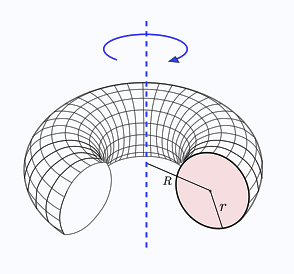
\includegraphics[height = 75mm]{teorGuldino.png}
		\caption{Rotazione di un dominio attorno all'asse \(z\).}
		\label{fig:teorGuldino}
	\end{centering}
\end{figure}

\begin{defn}{Trasformazione in coordinate sferiche}{coordSferiche}\index{Coordinate sferiche}
	Preso \((x,y,z)\in\R^3\setminus\{(0,0,z):z\in\R\}\), esiste una sola tripla \((\r,\j,\q)\in (0,+\infty)\times (0,\p)\times S^1\) tale che
	\[
		\begin{cases}
			x = \r \sin \j \cos \q \\
			y = \r \sin \j \sin \q \\
			z = \r \cos \j
		\end{cases}
	\]
	Rimane in tal modo individuato un diffeomorfismo \((x,y,z)\mapsto(\r,\j,\q)\) la cui funzione inversa è
	\[
		\y\colon(\r,\j,\q)\mapsto (x=\r\sin\j \cos\q,y=\r\sin\j \sin\q,z=\r\cos\j),
	\]
	detta \emph{trasformazione in coordinate sferiche}.
\end{defn}

\begin{oss}
	La figura \ref{fig:cordSfer} mostra una rappresentazione di un punto in coordinate sferiche.
\end{oss}

\begin{figure}[tp]
	\begin{centering}
		\includegraphics[height = 75mm]{cordSfer.pdf}
		\caption{Rappresentazione del passaggio da coordinate cartesiane a coordinate sferiche.}
		\label{fig:cordSfer}
	\end{centering}
\end{figure}

\begin{notz}
	\(\r,\j\) e \(\q\), che sono funzioni di \((x,y,z)\), si dicono \emph{coordinate sferiche} del punto di coordinate cartesiane \((x,y,z)\).
\end{notz}

\begin{prop}{Calcolo di un integrale mediante coordinate sferiche}{integraleCoordSferiche}
	Sia \(D\subseteq\R^3\) un dominio P-J misurabile e sia \(f\colon D\to\R\) una funzione R-integrabile.
	Se consideriamo \(\y^{-1}(D)\subseteq (0,+\infty)\times (0,\p)\times S^1\) il dominio la cui immagine tramite trasformazioni in coordinate sferiche è precisamente \(D\), allora vale
	\[
		\iiint\limits_D f(x,y,z)\,\dd x\,\dd y\,\dd z = \iiint\limits_{\y^{-1}(D)} f(\r\sin\j \cos\q,\r\sin\j \sin\q,\r \cos \j)\r^2\sin\j\,\dd \r\,\dd \j\,\dd \q.
	\]
\end{prop}

\begin{proof}
	La dimostrazione è analoga a quella per le coordinate sferiche e cilindriche, infatti
	\[
		\y\colon (0,+\infty)\times (0,\p)\times S^1 \to \R^3\setminus \{(0,0,z):z\in\R\},	\begin{pmatrix}
			\r \\
			\j \\
			\q
		\end{pmatrix}
		\mapsto	\begin{pmatrix}
			x = \r \sin \j \cos \q \\
			y = \r \sin \j \sin \q \\
			z = \r \cos \j
		\end{pmatrix}
	\]
	per cui
	\[
		\det \frac{\pd(x,y,z)}{\pd(\r,\j,\q)} = \abs*{\det 	\begin{pmatrix}
				\sin\j \cos\q & \r \cos\j \cos\q & -\r \sin\j \sin\q \\
				\sin\j \sin\q & \r \cos\j \sin\q & \r \sin\j \cos\q  \\
				\cos\j        & -\r \sin\j       & 0
			\end{pmatrix}}
		= \r^2 \sin\j
	\]
	dove \(\r^2 \sin\j\neq 0\) in quanto \(\r\in(0,+\infty)\) e \(\j\in (0,\p)\), ovvero ammette inversa \(C^1\) per il teorema della funzione inversa.
	Pertanto \(\y\) soddisfa le ipotesi del cambio di variabile.
	Per ottenere la tesi è quindi sufficiente considerare la restrizione di \(\y\) a \(D\).
\end{proof}

\begin{ese}
	Calcoliamo \(\abs{E}\) definito come il volume interno alla sfera
	\[
		\Set{(x,y,z) \in\R^3 | x^2+y^2+z^2 \le 2z}
	\]
	e sotto il paraboloide
	\[
		\Set{(x,y,z) \in \R^3 | z\le 2(x^2+y^2)}.
	\]
	Utilizziamo le coordinate sferiche:
	\[
		\y^{-1}(E) = \Set{(\r,\j,\q) | \q \in S^1, \r^2 \le 2\r \cos \j, \r \cos \j \le 2\r^2 \sin^2\j},
	\]
	ovvero
	\[
		\y^{-1}(E) = \Set{(\r,\j,\q) | \q \in S^1, \frac{\cos \j}{2 \sin^2\j} \le \r \le 2\cos \j}.
	\]
	Osserviamo che c'è una condizione implicita:
	\[
		\begin{split}
			\frac{\cos \j}{2\sin^2\j} \le 2\cos\j & \iff \frac{1}{4} \le \sin^2\j\\
			&  \iff \sin\j \ge \frac{1}{2}\\
			& \iff \j\in \left( \frac{\p}{6},\frac{\p}{2} \right),
		\end{split}
	\]
	dove abbiamo potuto dividere per \(\cos\j\) senza preoccuparci del segno in quanto \(\j\le \frac{\p}{2}\).
	Da cui, applicando le formule di riduzione,
	\[
		\begin{split}
			\int\limits_E \dd x\,\dd y\,\dd z & = \int\limits_{\y^{-1}(E)}\r^2 \sin\j \,\dd \r\,\dd \j\,\dd \q\\
			& = \int\limits_S^1 \dd \q \int_{\frac{\p}{6}}^{\frac{\p}{2}} \sin\j\,\dd \j \int_{\frac{\cos\j}{2\sin^2\j}}^{2\cos\j}\r^2\,\dd \r\\
			& = \frac{2}{3}\p \int_{\frac{\p}{6}}^{\frac{\p}{2}}\sin\j \left[ 8\cos^3\j- \frac{\cos^3\j}{8\sin^6\j} \right]\,\dd\j,
		\end{split}
	\]
	che è un integrale elementare.
\end{ese}
%%%%%%%%%%%%%%%%%%%%%%%%%%%%%%%%%%%%%%%%%%
%
%LEZIONE 23/03/2016 - QUINTA SETTIMANA (2)
%
%%%%%%%%%%%%%%%%%%%%%%%%%%%%%%%%%%%%%%%%%%
%%%%%%%%%%%%%%%%%%%%
%INTEGRALI IMPROPRI%
%%%%%%%%%%%%%%%%%%%%
\section{Integrali impropri}

In questo paragrafo ci occuperemo di definire l'integrale di funzioni non nulle su domini illimitati o di funzioni illimitate, ad esempio
\[
	\int_1^{+\infty}\frac{\dd x}{x^\a}\qquad\text{oppure}\qquad\int_0^1 \frac{\dd x}{x^\a}.
\]
Ricordiamo che nel caso monodimensionale potevamo scrivere
\[
	\lim_{R\to +\infty}\int_1^R \frac{\dd x}{x^\a}\qquad\text{e}\qquad \lim_{\e \to 0} \int_\e^1 \frac{\dd x}{x^\a},
\]
dove gli argomenti dei limiti sono funzioni R-integrabili.

\begin{defn}{Insieme illimitato Peano-Jordan misurabile}{peanoJordanIll}\index{Misura di Peano-Jordan!per insiemi illimitati}
	Sia \(A\subseteq \R^n\).
	Diremo che \(A\) è Peano-Jordan misurabile se \(A \cap B_r(\bar{0})\) è Peano-Jordan misurabile per ogni \(r>0\).
\end{defn}

\begin{oss}
	Se \(A\) è limitato, la definizione coincide con quella originale.

	Infatti \(A \cap B_r(\bar{0})\) è P-J misurabile se e soltanto se \(1_{A\cap B_r(\bar{0})}\) è R-integrabile.
	Ma \(1_{A\cap B_r(\bar{0})}=1_A \cdot 1_{B_r(\bar{0})}\), dove
	\[
		1_A \cdot 1_{B_r(\bar{0})} = 1_A,
	\]
	per \(r\) sufficientemente grande.
	Quindi \(1_A\) è R-integrabile se e soltanto se \(A\) è P-J misurabile.
\end{oss}

\begin{defn}{Funzione Riemann integrabile (caso positivo)}{RIntegrabilePos}
	Sia \(A\subseteq \R^n\) un insieme P-J misurabile anche illimitato.
	Diremo che \(f\colon A\to[0,+\infty)\) è Riemann integrabile su \(A\) se lo è, nel senso originale, su tutti i compatti P-J misurabili contenuti in \(A\) e se esiste finito
	\[
		\sup\Set{\int\limits_K f(x)\,\dd x | K\subseteq A, K\text{ compatto, P-J misurabile}}.
	\]
\end{defn}

\begin{notz}
	Se \(f\) è R-integrabile poniamo per definizione
	\[
		\int\limits_A f(x)\,\dd x = \sup\Set{\int\limits_K f(x)\,\dd x | K\subseteq A, K\text{ compatto, P-J misurabile}}.
	\]
\end{notz}

\begin{oss}
	Sui compatti \(K\subseteq A\) P-J misurabili \(f\) è R-integrabile, in particolare sarà limitato.
	Pertanto eventuali asintoti verticali di \(f\) si trovano necessariamente sul bordo di \(A\).
\end{oss}

\begin{oss}
	Se \(A\) è limitato e \(f\) è R-integrabile su \(A\), la definizione si riconduce a quella originale.

	Questo è banalmente vero nel caso che \(A\) sia compatto, mentre nel caso non lo fosse è sufficiente ricoprire \(A\) dall'interno con polirettangoli compatti.
\end{oss}

\begin{ese}
	Questa definizione è problematica con funzione che assumono valori negativi.
	Consideriamo ad esempio,
	\[
		\int_0^{+\infty}\frac{\sin x}{x}\,\dd x,
	\]
	Che sappiamo, per l'analisi monodimensionale, essere convergente.
	Per la definizione appena data avremo
	\[
		\int_0^{+\infty}\frac{\sin x}{x}\,\dd x \overset{\text{def}}{=} \int_0^{+\infty} \left( \frac{\sin x}{x} \right)^+\,\dd x.
	\]
	Possiamo vedere nella figura \ref{fig:impr1} come la funzione sia positiva in intervalli di ampiezza \(\p\).
	Da cui
	\[
		\begin{split}
			\int_0^{+\infty} \left(\frac{\sin x}{x}\right)^+\,\dd x & = \lim_{n\to +\infty} \int_0^{2\p\,n} \left( \frac{\sin x}{x} \right)^+\,\dd x\\
			& = \lim_{n\to +\infty}\sum_{i=0}^{n-1} \int_{2i\,\p}^{(2i+1)\p} \frac{\sin x}{x}\,\dd x\\
			& \ge \lim_{n\to +\infty} \sum_{i=0}^{n-1} \int_{2i\,\p}^{(2i+1)\p} \frac{\sin x}{(2i+1)\p}\,\dd x\\
			& = \lim_{n\to +\infty}\sum_{i=0}^{n-1} \frac{2}{(2i+1)\p} = +\infty.\graffito{per la divergenza della serie armonica tramite il criterio di condensazione}
		\end{split}
	\]
	Quindi questa definizione di integrale improprio si comporta più come l'integrale del modulo.
\end{ese}

\begin{figure}[tp]
	\begin{centering}
		\includegraphics[height = 75mm]{impr1.pdf}
		\caption{La funzione \(\frac{\sin x}{x}\) evidenziata nella regione positiva.}
		\label{fig:impr1}
	\end{centering}
\end{figure}

\begin{defn}{Funzione Riemann integrabile (caso generale)}{RIntegrabileGen}
	Sia \(A\subseteq\R^n\) un insieme P-J misurabile anche illimitato.
	Diremo che \(f\colon A \to \R\) è Riemann integrabile se lo sono \(f^+\) e \(f^-\).
	In tal caso poniamo
	\[
		\int\limits_A f(x)\,\dd x = \int\limits_A f^+(x)\,\dd x -\int\limits_A f^-(x)\,\dd x.
	\]
\end{defn}

\begin{oss}
	Gli integrali su \(A\) di \(f^+\) e \(f^-\) sono entrambi finiti perché abbiamo chiesto che siano R-integrabili.
\end{oss}

\begin{prop}{R-integrabilità del modulo di una funzione}{RIntegrabileMod}
	Sia \(A\) un insieme P-J misurabile e sia \(f\colon A \to \R\).
	Allora \(f^+,f^-\) sono R-integrabili se e soltanto se \(\abs{f}\) è R-integrabile.
\end{prop}

\begin{proof}
	\graffito{\(\Rightarrow)\)}Per definizione
	\[
		\abs*{f(x)} = f^+(x)+f^-(x),
	\]
	per cui \(\abs{f}\) è R-integrabile per la linearità dell'integrale.

	\graffito{\(\Leftarrow)\)}Segue da
	\[
		\abs*{f(x)} \ge 	\begin{cases}
			f^+(x) \\
			f^-(x)
		\end{cases}\qedhere
	\]
\end{proof}

\begin{oss}
	Quindi, per quanto mostrato nell'esempio precedente, la funzione \(\frac{\sin x}{x}\) non è R-integrabile su \((0,+\infty)\), infatti
	\[
		\int_0^{+\infty} \abs*{\frac{\sin x}{x}}\,\dd x = +\infty.
	\]
\end{oss}

\begin{prop}{Confronto integrale}{confrontoIntegrale}
	Sia \(A\subseteq\R^n\) un insieme P-J misurabile e consideriamo \(f\colon A\to \R,g\colon A\to [0,+\infty)\).
	Supponiamo che \(f\) sia R-integrabile su ogni compatto P-J misurabile contenuto in \(A\) e che \(g\) sia R-integrabile.
	Se
	\[
		\abs*{f(x)} \le g(x),\,\fa x\in A,
	\]
	allora \(f\) è R-integrabile e vale
	\[
		\int\limits_A \abs*{f(x)}\,\dd x \le \int\limits_A g(x)\,\dd x.
	\]
\end{prop}

\begin{proof}
	Affinchè \(f\) sia R-integrabile dobbiamo mostrare che l'estremo superiore dell'integrale su tutti i compatti contenuti in \(A\) è finito.
	Dal momento che \(f\) è R-integrabile su ogni compatto \(K\subseteq A\) P-J misurabile, avremo
	\[
		\int\limits_K \abs*{f(x)}\,\dd x \le \int\limits_K g(x)\,\dd x,
	\]
	da cui
	\[
		\sup_{K\subseteq A} \int\limits_K \abs*{f(x)}\,\dd x \le \sup_{K\subseteq A} \int\limits_K g(x)\,\dd x = \int\limits_A g(x)\,\dd x.\qedhere
	\]
\end{proof}

\begin{teor}{Limite sui compatti per l'integrale improprio}{limiteIntImproprio}
	Sia \(A\subseteq\R^n\) un insieme P-J misurabile e sia \(\{K_j\}\) una catena crescente di compatti P-J misurabili contenuti in \(A\), tali che per ogni compatto \(K\subseteq A\) esiste \(K_j\supseteq K\).

	Allora
	\[
		\lim_{j\to +\infty} \int\limits_{K_j}\abs{f(x)}\,\dd x <+\infty \iff f \text{ è integrabile su }A,
	\]
	e risulta
	\[
		\int\limits_A \abs{f(x)}\,\dd x = \lim_{j\to +\infty}\int\limits_{K_j}f(x)\,\dd x.
	\]
\end{teor}

\begin{proof}
	\graffito{\(\Leftarrow)\)}Supponiamo che \(f\) sia integrabile su \(A\), quindi \(\abs{f}\) è integrabile, da cui
	\[
		\int\limits_A \abs*{f(x)}\,\dd x \le \sup\Set{\int\limits_K \abs*{f(x)}\,\dd x | K\subseteq A, K\text{ compatto, P-J misurabile}}<+\infty.
	\]
	In particolare ogni \(K_j\) è un compatto, P-J misurabile, contenuto in \(A\), quindi
	\[
		\int\limits_{K_j}\abs*{f(x)}\,\dd x \le \int\limits_A \abs{f(x)}\,\dd x,\,\fa j,
	\]
	ovvero
	\[
		\lim_{j\to +\infty}\int\limits_{K_j}\abs*{f(x)}\,\dd x \le \int\limits_A \abs*{f(x)}\,\dd x < +\infty.
	\]
	\graffito{\(\Rightarrow)\)}Sia \(K\subseteq A\) un compatto P-J misurabile.
	Per ipotesi esiste \(K_j \supseteq K\), quindi, per la monotonia dell'integrale,
	\[
		\int\limits_K \abs*{f(x)}\,\dd x \le \int\limits_{K_j}\abs*{f(x)}\,\dd x,\text{ con \(j\) sufficientemente grande},
	\]
	da cui
	\[
		\int\limits_K \abs*{f(x)}\,\dd x \le \lim_{j\to +\infty} \int\limits_{K_j}\abs*{f(x)}\,\dd x,\,\fa k.
	\]
	In particolare, per definizione di estremo superiore,
	\[
		\sup\Set{\int\limits_K \abs*{f(x)}\,\dd x | K\subseteq A, K\text{ compatto, P-J misurabile}} \le \lim_{j\to +\infty}\int\limits_{K_j} \abs*{f(x)}\,\dd x < +\infty,
	\]
	ovvero
	\[
		\int\limits_A \abs*{f(x)}\,\dd x \le \lim_{j\to +\infty} \int\limits_{K_j} \abs*{f(x)}\,\dd x.
	\]
	Resta da dimostrare che l'integrale di \(f\) su \(A\) corrisponde precisamente al limite sui \(K_j\).
	Per quanto appena dimostrato sappiamo che\graffito{le due frecce lo dimostrano per doppia disuguaglianza}
	\[
		\lim_{j\to +\infty}\int\limits_{K_j}\abs*{f(x)}\,\dd x = \int\limits_A \abs*{f(x)}\,\dd x.
	\]
	Applicando lo stesso ragionamento a \(f^+\) e \(f^-\), che sono anch'esse funzioni positive, avremo
	\[
		\lim_{j\to +\infty}\int\limits_{K_j}f^+(x)\,\dd x = \int\limits_A f^+(x)\,\dd x \qquad\text{e}\qquad \lim_{j\to +\infty}\int\limits_{K_j}f^-(x)\,\dd x = \int\limits_A f^-(x)\,\dd x.
	\]
	Quindi, per la linearità del limite,
	\[
		\begin{split}
			\lim_{j\to +\infty}\int\limits_{K_j}f(x)\,\dd x & = \lim_{j\to +\infty} \left[ \int\limits_{K_j}f^+(x)\,\dd x - \int\limits_{K_j}f^-(x)\,\dd x \right]\\
			& = \lim_{j\to +\infty} \int\limits_{K_j}f^+(x)\,\dd x - \lim_{j\to +\infty} \int\limits_{K_j}f^-(x)\,\dd x\\
			& = \int\limits_A f^+(x)\,\dd x - \int\limits_A f^-(x)\,\dd x = \int\limits_A f(x)\,\dd x.\qedhere
		\end{split}
	\]
\end{proof}

\begin{ese}
	Troviamo per quali \(\a\) vale
	\[
		\int\limits_A \frac{\dd x\,\dd y}{\abs{x-y}^\a} < +\infty,
	\]
	dove
	\[
		A = \Set{(x,y)\in\R^2 | x \in [0,1], y \in [0,1], x\neq y}.
	\]
	Sicuramente per \(\a \le 0\) avremo l'integrabilità in quanto la funzione è limitata su \(A\).
	Se \(\a>0\) l'integrale è improprio in quanto la funzione integranda tende all'infinito lungo la diagonale.

	Osserviamo dalla figura \ref{fig:impr2} che \(A=A'\cup A''\) con \(A'=A''\).
	Possiamo quindi scrivere
	\[
		\int\limits_A \frac{\dd x\,\dd y}{\abs{x-y}^\a} = 2 \int\limits_{A'} \frac{\dd x\,\dd y}{\abs{x-y}^\a}.
	\]
	Per applicare il teorema devo trovare una catena di compatti che ricoprano \(A'\) su cui la funzione è R-integrabile.
	Consideriamo quindi tutti gli insiemi in \(A'\) privi della diagonale, ovvero
	\[
		K_j = \Set{(x,y)\in\R^2 | 0 \le x \le 1- \frac{1}{j}, x+ \frac{1}{j} \le y \le 1}.
	\]
	Applicando il teorema e le formule di riduzione avremo
	\[
		\begin{split}
			2\int\limits_{A'} \frac{\dd x\,\dd y}{\abs{x-y}^\a} & = 2\lim_{j\to +\infty} \int\limits_{K_j} \frac{\dd x\,\dd y}{\abs{x-y}^\a}\\
			& = 2\lim_{j\to +\infty} \int_0^{1- \frac{1}{j}}\dd x \int_{x+ \frac{1}{j}}^1 \frac{\dd y}{(y-x)^\a}\graffito{se \(\a\neq 1\)}\\
			& = 2\lim_{j\to +\infty} \int_0^{1- \frac{1}{j}} \left[ \frac{(y-x)^{1+\a}}{1-\a} \right]_{x+ \frac{1}{j}}^1\,\dd x\\
			& = \frac{2}{1-\a} \lim_{j\to +\infty} \int_0^{1- \frac{1}{j}} (1-x)^{1-\a}- \left( \frac{1}{j} \right)^{1-\a}\,\dd x\graffito{se \(\a\neq 2\)}\\
			& = \frac{2}{1-\a} \lim_{j\to +\infty} \left[ - \frac{(1-x)^{2-\a}}{2-\a}-x \left( \frac{1}{j} \right)^{1-\a} \right]_0^{1- \frac{1}{j}}\\
			& = \frac{2}{1-\a} \lim_{j\to +\infty} \left[ -\frac{1}{2-\a}\left( \frac{1}{j} \right)^{2-\a}+\frac{1}{2-\a}-\left( 1- \frac{1}{j} \right) \left( \frac{1}{j} \right)^{1-\a} \right],
		\end{split}
	\]
	quindi la funzione è integrabile su \(A\) per \(\a<1\).\graffito{i casi \(\a=1,2\) andrebbero gestiti separatamente}
\end{ese}

\begin{figure}[tp]
	\begin{centering}
		\includegraphics[height = 75mm]{impr2.pdf}
		\caption{Il dominio \(A\) ed una visualizzazione dei compatti \(K_j\).}
		\label{fig:impr2}
	\end{centering}
\end{figure}

\begin{ese}
	Presa una matrice simmetrica \(A\) vogliamo calcolare
	\[
		\int\limits_{\R^n}e^{-\frac{\Braket{x,A\,x}}{2}}\,\dd x.
	\]
	Nel caso particolare in cui \(A\) è diagonale,
	\[
		A = 	\begin{pmatrix}
			\l_1   & \dots  & 0      \\
			\vdots & \ddots & \vdots \\
			0      & \dots  & \l_n
		\end{pmatrix}
	\]
	e sapendo
	\[
		\int\limits_{\R^n} e^{-\frac{x^2}{2t}}\,\dd x = \sqrt{2\p\,t},t>0,
	\]
	avremo
	\[
		\begin{split}
			\int\limits_{\R^n}e^{-\frac{\Braket{x,A\,x}}{2}}\,\dd x & = \int\limits_{\R^n}e^{-\l_1 \frac{x_1^2}{2}}\ldots e^{-\l_n \frac{x_n^2}{2}}\,\dd x_1\,\ldots\,\dd x_n\\
			& = \int\limits_\R e^{-\l_1 \frac{x_1^2}{2}}\,\dd x_1 \ldots \int\limits_\R e^{-\l_n \frac{x_n^2}{2}}\,\dd x_n\\
			& = \frac{\sqrt{(2\p)^n}}{\sqrt{\l_1 \cdot\ldots\cdot \l_n}} = \frac{\sqrt{(2\p)^n}}{\sqrt{\det A}}.
		\end{split}
	\]
	Vogliamo generalizzare questo procedimento sfruttando la diagonalizzazione di \(A\).
	Infatti \(A\) simmetrica ci garantisce che \(A=B^{-1}D\,B\) con \(D\) diagonale, per cui
	\[
		\int\limits_{\R^n} e^{- \frac{\Braket{A\,x,x}}{2}}\,\dd x = \int\limits_{\R^n} e^{-\frac{\Braket{B^{-1}D\,B\,x,x}}{2}}\,\dd x,
	\]
	dove \(B\) è ortogonale, per cui \(B^{-1}={}^{t}B\), quindi
	\[
		\frac{\Braket{B^{-1} D\,B\,x,x}}{2} = \frac{\Braket{D\,B\,x,B\,x}}{2}.
	\]
	Applichiamo il cambio di variabile \(y=B\,x\), per cui \(x=B^{-1}\,y \implies \dd x = \det B^{-1}\,\dd y\).
	Ma \(B^{-1}\) è una rotazione, per cui \(\det B^{-1} = 1\), ovvero \(\dd x = \dd y\).
	Applicato all'integrale otteniamo
	\[
		\int\limits_{\R^n} e^{-\frac{\Braket{D\,y,y}}{2}}\,\dd y = \frac{\sqrt{(2\p)^n}}{\sqrt{\det D}} = \frac{\sqrt{(2\p)^n}}{\sqrt{\det A}},
	\]
	in quanto
	\[
		\det A = \det(B^{-1}D\,B) = \frac{1}{\det B}\det D\,\det B = \det D.\qedhere
	\]
\end{ese}